
%%%%%%%%%%%%%%%%%%%%%%%%%%%%%%%%%%%%%%%%%%%%%%%%%%%%%%%%%%%%%%%%%%%%%%%%%%%%
%%%%%%%%%%%%%%%%%%%%%%%%%%%%%%%%%%%%%%%%%%%%%%%%%%%%%%%%%%%%%%%%%%%%%%%%%%%%
%%%%%%%%%%%%%%%%%%%%%%%%%%%%%%%%%%%%%%%%%%%%%%%%%%%%%%%%%%%%%%%%%%%%%%%%%%%%

\begin{frame}[t]{Which estimators do we study?}

Suppose we have $N$ data points $\d_{1}, \ldots, \d_{N}$.  Then:
%
\begin{align*}
%
\thetahat \only<2->{\color{red} (\w) \color{black}} :=
\vec\theta \,\, \textrm{ such that } \,\,
\sumn
\only<2->{ \color{red} \w_{n} \color{black}}
G(\vec\theta, \d_{n}) =  \zP .
%
\end{align*}
%
\onslide<1->{
Leave points out by setting their elements of $\w$ to zero.
}

\onslide<1->{
These are ``Z-estimators,'' i.e., roots of estimating equations.

Examples: all minimizers of empirical loss (OLS, MLE, VB), and more.
}


\end{frame}



%%%%%%%%%%%%%%%%%%%%%%%%%%%%%%%%%%%%%%%%%%%%%%%%%%%%%%%%%%%%%%%%%%%%%%%%%%%%
%%%%%%%%%%%%%%%%%%%%%%%%%%%%%%%%%%%%%%%%%%%%%%%%%%%%%%%%%%%%%%%%%%%%%%%%%%%%
%%%%%%%%%%%%%%%%%%%%%%%%%%%%%%%%%%%%%%%%%%%%%%%%%%%%%%%%%%%%%%%%%%%%%%%%%%%%


\begin{frame}[t]{Which estimators do we study?}

Suppose we have $N$ data points $\d_{1}, \ldots, \d_{N}$.  Then:
%
\begin{align*}
%
\thetahat(\w) :=
\vec\theta \,\, \textrm{ such that } \,\,
\sumn
\w_{n} G(\vec\theta, \d_{n}) =  \zP .
%
\end{align*}
%
{
Leave points out by setting their elements of $\w$ to zero.
}

\onslide<2->{
\hrulefill
}
%
%
% \vspace{1em}

Fix a quantity of interest, $\phi(\vec\theta)$.

Let the \textbf{``signal''}, $\Delta$, be a ``large'' change in $\phi$.

\begin{columns}
%
\begin{column}{0.45\linewidth}
    \onslide<2->{
    Examples:
    %
    \begin{align*}
        \phi(\vec\theta) =&{} \vec\theta_p\\
        \phi(\vec\theta) =&{} \vec\theta_p +
            \frac{1.96}{\sqrt{N}} \hat\sigma_\phi(\vec\theta)
    \end{align*}
    }
\end{column}
%
\begin{column}{0.45\linewidth}
    \onslide<4->{
    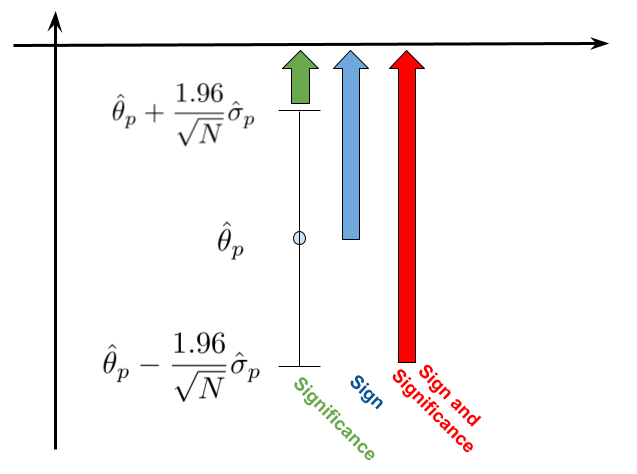
\includegraphics[width=0.95\linewidth]{static_figures/adversarial_robustness_example_phi_flipped.png}
    }
\end{column}
\end{columns}


\end{frame}


%%%%%%%%%%%%%%%%%%%%%%%%%%%%%%%%%%%%%%%%%%%%%%%%%%%%%%%%%%%%%%%%%%%%%%%%%%%%
%%%%%%%%%%%%%%%%%%%%%%%%%%%%%%%%%%%%%%%%%%%%%%%%%%%%%%%%%%%%%%%%%%%%%%%%%%%%
%%%%%%%%%%%%%%%%%%%%%%%%%%%%%%%%%%%%%%%%%%%%%%%%%%%%%%%%%%%%%%%%%%%%%%%%%%%%


\begin{frame}[t]{Which estimators do we study?}

Suppose we have $N$ data points $\d_{1}, \ldots, \d_{N}$.  Then:
%
\begin{align*}
%
\thetahat(\w) :=
\vec\theta \,\, \textrm{ such that } \,\,
\sumn
\w_{n} G(\vec\theta, \d_{n}) =  \zP .
%
\end{align*}
%
Leave points out by setting their elements of $\w$ to zero.

\hrulefill

%\vspace{1em}
%
Fix a quantity of interest, $\phi(\vec\theta)$.

Let the \textbf{``signal''}, $\Delta$, be a ``large'' change in $\phi$.

\hrulefill

Can we reverse our conclusion by dropping $\lfloor \alpha N \rfloor$
datapoints? \pause

\vspace{1em}
$\Leftrightarrow$
\vspace{1em}

Is there a $\w$, with
$\lfloor \alpha N \rfloor$ zeros, such that
$\thetafun(\thetahat(\w)) - \thetafun(\thetahat) \ge \Delta$?

\vspace{1em}

\textbf{Hard!}
Evaluating $\thetahat(\w)$ is costly and lots of $\w$
have $\lfloor \alpha N \rfloor$ zeros.

% To simplify the search over $\w$, we will approximate
% $\w \mapsto \thetafun(\thetahat(\w))$.

\end{frame}


%%%%%%%%%%%%%%%%%%%%%%%%%%%%%%%%%%%%%%%%%%%%%%%%%%%%%%%%%%%%%%%%%%%%%%%%%%%%
%%%%%%%%%%%%%%%%%%%%%%%%%%%%%%%%%%%%%%%%%%%%%%%%%%%%%%%%%%%%%%%%%%%%%%%%%%%%
%%%%%%%%%%%%%%%%%%%%%%%%%%%%%%%%%%%%%%%%%%%%%%%%%%%%%%%%%%%%%%%%%%%%%%%%%%%%


\begin{frame}{Taylor series approximation.}
%
Is there a $\w$, with
$\lfloor \alpha N \rfloor$ zeros, such that
$\thetafun(\thetahat(\w)) - \thetafun(\thetahat) \ge \Delta$?

\vspace{-0.5em}
\hrulefill

To simplify the search over $\w$, we form the Taylor series approximation:
%
\begin{align*}
	\thetafun(\thetahat(\w)) - \thetafun(\thetahat)
		&\approx
        \color{red}
        \thetafunlin(\w) - \thetafun(\thetahat)
        \color{black}
		:=  -
        \sum_{n: \w_n = 0} \infl_n
        \color{black}
\textrm{, where }
\infl_n := \fracat{\partial \thetafun(\thetahat(\w))}{\partial \w_n}{\onevec}.
\end{align*}
%
\pause
The values $\infl_n$ are the
\textbf{``empirical influence function.''}
%\citep{hampel1986robustbook}
{\footnotesize \citep{hampel1986robustbook}}

The $\infl_n$ can be \textbf{easily
and automatically} computed from $\thetahat$.

The approximation is
\textbf{typically accurate}
for small $\alpha$.

\pause
\vspace{-0.5em}
\hrulefill

Is there a $\w$, with
$\lfloor \alpha N \rfloor$ zeros, such that
$\color{red} \thetafunlin(\w) - \thetafun(\thetahat) \color{black} \ge \Delta$?

\pause
\vspace{1em}

\textbf{Easy!}
The most influential points for $\thetafunlin(\w)$ have the most negative
$\infl_n$.

\end{frame}






%%%%%%%%%%%%%%%%%%%%%%%%%%%%%%%%%%%%%%%%%%%%%%%%%%%%%%%%%%%%%%%%%%%%%%%%%%%%
%%%%%%%%%%%%%%%%%%%%%%%%%%%%%%%%%%%%%%%%%%%%%%%%%%%%%%%%%%%%%%%%%%%%%%%%%%%%
%%%%%%%%%%%%%%%%%%%%%%%%%%%%%%%%%%%%%%%%%%%%%%%%%%%%%%%%%%%%%%%%%%%%%%%%%%%%


\begin{frame}{Taylor series approximation.}

\textbf{Procedure:}

\begin{enumerate}
    \item<2-> Compute the ``original'' estimator, $\thetahat$ and
    $\thetafun(\thetahat)$.
    \item<3-> Compute and sort the influence scores,
        $\infl_{(1)} \le \infl_{(2)} \le \ldots \le \infl_{(N)}$.
    \item<4-> Let $\w^*$ leave out the data corresponding to
    $\infl_{(1)},  \ldots , \infl_{(\lfloor \alpha N \rfloor)}$.
    %the $\lfloor \alpha N \rfloor$ most negative influence scores.
    \item<5-> Report non-robustness if
        $ \Delta \le \thetafunlin(\w^*) - \thetafun(\thetahat)  =
            - \sum_{n=1}^{\lfloor \alpha N \rfloor} \infl_{(n)}$.
    \item<6-> \textbf{Optional: } Compute $\thetahat(\w^*)$, and verify
    that $\Delta \le \thetafun(\thetahat(\w^*)) - \thetafun(\thetahat)$.
\end{enumerate}

% \onslide<7->{
% We have an \texttt{R} package, \texttt{rgiordan/zaminfluence},
%     for OLS and IV.}

% \onslide<7->{
% \textbf{The above procedure can be automated using:}
% }
%
%
% \begin{itemize}
%     \item<8-> Code to compute $G(\theta, \d_n)$ and $\thetafun$,
%     \item<9-> The ``base solution'' $\thetahat(\onevec)$, and
%     \item<10-> Automatic differentiation. \citep{baydin2017automatic}
%     \item<11-> E.g., our \texttt{R} package, \texttt{rgiordan/zaminfluence}
%         for OLS and IV
% \end{itemize}


\end{frame}




%%%%%%%%%%%%%%%%%%%%%%%%%%%%%%%%%%%%%%%%%%%%%%%%%%%%%%%%%%%%%%%%%%%%%%%%%%%%
%%%%%%%%%%%%%%%%%%%%%%%%%%%%%%%%%%%%%%%%%%%%%%%%%%%%%%%%%%%%%%%%%%%%%%%%%%%%
%%%%%%%%%%%%%%%%%%%%%%%%%%%%%%%%%%%%%%%%%%%%%%%%%%%%%%%%%%%%%%%%%%%%%%%%%%%%


\begin{frame}{Computing the influence function.}

How to compute
$\infl_n := \fracat{\partial \thetafun(\thetahat(\w))}{\partial \w_n}{\onevec}$?
%
Recall $\sumn \w_{n} G(\thetahat(\w), \d_{n}) =  \zP$.

\textbf{Step zero:}
Implement software to compute $G(\theta, \d_{n})$ and
$\thetafun(\theta)$. Find $\thetahat$.

\textbf{Step one:}
By the chain rule,
$\infl_n = \fracat{\partial \thetafun(\thetahat(\w))}{\partial \w_n}{\onevec}
= \fracat{\dee \thetafun(\theta)}
    {\dee \theta^T}{\thetahat}
  \fracat{\partial \thetahat(\w)}{\partial \w_n}{\onevec}$.

\textbf{Step two:}
By the implicit function theorem:
%
\begin{align*}
%
\fracat{\partial \thetahat(\w)}{\partial \w_n}{\onevec} ={}
\frac{1}{N}
\left(
  \frac{1}{N}
  \sum_{n'=1}^N
    \frac{\partial}{\partial \theta^T} G(\vec\theta, \d_{n'})
        \Big\vert_{\thetahat}
\right)^{-1} G(\thetahat, \d_{n}).
%
\end{align*}
%

\textbf{Step three:}
%
Use \textit{automatic differentiation} on $\phi(\theta)$ and $G(\theta, \d_{n})$
from step zero to compute $\frac{\partial \thetafun(\theta)}{\partial \theta^T}$
and $\frac{\partial}{\partial \theta^T} G(\vec\theta, \d_{n})$.
% Put the pieces together.

\hrulefill

\begin{itemize}
    \item The user does step zero.  The rest is automatic.
    \item The primary computational expense is the Hessian inverse.
    \item Automatic differentiation is the chain rule applied to a program.
     %(not symbolic, nor numerical).
    \item Typically $\infl_n = O(N^{-1})$.
    %\item Note that $\infl_n  = O_p(N^{-1})$ by step two (typically).
\end{itemize}


% \onslide<7->{
% We have an \texttt{R} package, \texttt{rgiordan/zaminfluence},
%     for OLS and IV.}

% \onslide<7->{
% \textbf{The above procedure can be automated using:}
% }
%
%
% \begin{itemize}
%     \item<8-> Code to compute $G(\theta, \d_n)$ and $\thetafun$,
%     \item<9-> The ``base solution'' $\thetahat(\onevec)$, and
%     \item<10-> Automatic differentiation. \citep{baydin2017automatic}
%     \item<11-> E.g., our \texttt{R} package, \texttt{rgiordan/zaminfluence}
%         for OLS and IV
% \end{itemize}


\end{frame}
